%\documentstyle[a4j,epsbox,graphicx]{jarticle}
\documentclass[a4j]{jarticle}%変更禁止!
%%%%%%%%%%%%usepackageは適宜追加してください.%%%%%%%%%%%%%%%%%%%%%%%%%%%%%%%%%%%%%%%%%%%%%%%%%%%
%\usepackage{epsbox}
%\usepackage{graphicx}
\usepackage[dvipdfmx]{graphicx,color}
%%%%%%%%%%%%%%%%%%%%%%%%%%%ここから変更禁止%%%%%%%%%%%%%%%%%%%%%%%%%%%%%%%%%%%%%%%%%%%%%%%%%%
\topmargin -28mm
\oddsidemargin -15mm
\evensidemargin -15mm
\textwidth 185mm
\textheight 275mm
\columnsep 6mm

%\def\toujitu{Dec. 2019}

\makeatletter
\def\section{\@startsection{section}{2}{\z@}{.8ex plus .8ex minus 
 .2ex}{.05ex plus .07ex}{\large\bf}}
\makeatother
\makeatletter
\def\subsection{\@startsection{subsection}{2}{\z@}{.8ex plus .8ex minus 
 .2ex}{.05ex plus .07ex}{\bf}}
\makeatother


\pagestyle{empty}

\begin{document}

\baselineskip 4.75mm

\twocolumn
[
\footnotesize 
\begin{center}
{~}\\
%\begin{center}
%{ユビキタスウェアラブルワークショップ2019 
%\hfill \toujitu}\\
%%%%%%%%%%%%%%%%%%%%%%%%%%%ここまで変更禁止%%%%%%%%%%%%%%%%%%%%%%%%%%%%%%%%%%%%%%%%%%%%%%%%%%

%%%注意!!\vspaceは図表部分のみ見にくく(醜く)ならない範囲内で使用可能とします.%%%%%%%%%%%%%%%%%%%%%%%%%%%%

\medskip
{\large
%タイトル
{\bf 圧力センサ搭載ヘルメットを用いた個人識別手法の提案}\\
}
\medskip
{\large
%著者 同じ所属の人が連続する場合は連続する同じ所属の著者の最後の著者のみに所属を付けること.
         藤井敦寛(立命館大学),村尾和哉(立命館大学,JSTさきがけ)
}
\end{center}
]

\section{研究の背景と目的}
%現代の四輪車にキーレスエントリーシステムが導入されていることが多い.キーレスエントリーシステムとは,四輪車のドアに備え付けられている鍵穴に鍵を挿し込むことなく,リモートコントローラでドアのロックやアンロックがボタン1つで可能なシステムである.しかし,エンジンの始動には備え付けの鍵を挿す必要がある.近年はエンジンの始動もキーレスでできるスマートキーシステムの開発が行われている.しかし,これらのシステムは鍵の紛失によって所有者以外の人物によって利用される可能性がある.したがって,これらのシステムでは所有者の認証方法がセキュリティ的に重要であるといえる.\par
%近年販売されている四輪車にキーレスシステムやスマートキーシステムを導入している事例が多い.しかし,二輪車にこれらのシステムを導入している事例は少ない.そこで,本研究では二輪車のスマートキーシステムを普及させるための初期段階として,ヘルメットを用いた個人識別手法を提案する.現在,日本国内の公道を走行するためにヘルメットの着用が義務付けられている.そのため,ヘルメットを鍵の代用として用いることで簡単にスマートキーシステムを導入することができると考えられる.提案手法はヘルメットを装着した際に取得できる装着者の頭部形状を用いて個人を識別する.識別方法は個人の特徴が存在し,複製が難しいような方法が適している.白川らは虹彩と目の周辺画像を統合し認証する手法を提案している\cite{bib1}.しかし,目とその周辺画像の取得に目前に設置したカメラが必要である.カメラをヘルメットなどの二輪車に関係した部品に取り付けることは取り付け場所や費用の問題がある.提案手法で用いる頭部形状は個人差が存在しており,かつ複製することが難しい.そのため,識別方法に適していると考えられる.また,ヘルメットを用いることで新たに部品を取り付ける必要がない.
%ここまでM1チェック時に考案した文章,以下提出時の原文
現在スマートカーが注目され,四輪車におけるキーレス化の開発が進む中で,二輪車でのキーレス化は普及していない.そこで二輪車におけるキーレス化に向け,ヘルメットを用いた個人識別手法を提案する.日本国内の公道走行ではヘルメットの着用が義務付けられており,乗車する上で必要な物であるため,これを鍵の代わりに用いる.認証に用いる要素には個人により特徴があり,また偽装が難しいことが重要である.白川らは虹彩と目の周辺画像を統合し認証する手法を提案している\cite{bib1}.しかし,目とその周辺画像の取得には目前にカメラが必要であり,ヘルメットに応用するのは難しいため,本研究では個人識別に頭部形状を用いる.ヘルメットを被った際に頭部形状が取得できれば,その差異から個人を識別することが可能であると予想できる.また頭部形状は複製が難しく,認証に適していると考えた.

\section{提案手法}
%提案手法は所有者が普段着用するヘルメットにセンサを取り付ける.ヘルメットを着用してから2[ms]のセンサ値データを入力データとして,事前に収集しておいた所有者本人のデータと照合して個人識別をする.センサ値データは32個のセンサから得られる電圧値データを要素とするベクトルである.これらのベクトルは主成分分析によって32次元から2次元に削減する.事前に収集しておいたデータの重心を計算しておき,未知のデータの重心との距離を計算する.計算結果を用いて,所有者本人がヘルメットを着用しているか閾値で判断する.
%ここまでM1チェック時に考案した文章,以下提出時の原文
ヘルメットを被った状態で2[ms]静止し,その間のセンサ値をデータとして蓄積していく.このデータは32個の電圧値を要素とするベクトルであるが,識別に必要なデータは1回被った時に1ベクトルのみであるため,この2[ms]のデータの平均値を用いることとする.また外れ値の影響を考慮し,この32次元ベクトルは主成分分析を行い,2次元に削減する.識別ではデータセットの中で学習データに用いる個数を設定し,学習データの重心を計算する.鍵としての識別ではヘルメットの持ち主であるか,そうでないかを判別するのみであるため,単純に重心から認証データに対する距離により,閾値を用いて判別する.

\section{実装}
実装したプロトタイプデバイスを図\ref{device}に示す.図\ref{device}の左図はプロトタイプデバイスの全体図である.センサ値を正しく取得するには,センサとヘルメット装着者の頭部が密着している必要がある.そのため,フルフェイス型のB\&B社製BB100フルフェイスヘルメットを用いた.ヘルメット内部にはインターリンク エレクトロニクス社製の圧力センサであるFSR402,FSR402 ShortTailを取り付けた.圧力センサは全て並列接続であり,ヘルメット外部に取り付けた10KΩの抵抗を配線してあるプリント基板を経由して,マイコンであるArduino MEGA2560 R3のアナログ入力ポートに接続した.
%実装したプロトタイプデバイスを図\ref{device}に示す.図\ref{device}の左図はデバイスの全体図である.ヘルメット(B\&B社製BB100フルフェイスヘルメット)内部に圧力センサ(インターリンク エレクトロニクス社製FSR402,FSR402 ShortTail)を取り付けている.センサは全て並列接続でヘルメット外部のプリント基板上で抵抗(10KΩ)を配線し,マイコン(Arduino MEGA2560 R3)のアナログ入力ポートと接続している.\par
図\ref{device}の右図はヘルメット内部の様子である.今回用いたヘルメットがフリーサイズで少し大きめであり,内装の脱着が不可能であった.そのため,頭頂部の内装を取り外して,新たに厚みのあるウレタンスポンジを取り付けた.取り付けたウレタンスポンジの中央部に切り込みを入れ,切り込み部分に圧力センサを挿し込んだ.圧力センサは頭頂部に4個,頭頂部周囲に16個,後頭部に6個,左右チークパッド部に6個の合計32個を搭載した.
%図\ref{device}の右図はヘルメット内部である.センサ値を取得するためには,可能な限り頭部と密着している必要がある.そのため,フルフェイスヘルメットを選択した.しかしこのヘルメットはフリーサイズであり少し大きめの作りだったこと,内装の脱着が不可能だったことから頭頂部の内装を剥がし,新たに厚みのあるウレタンスポンジを貼り付けた.このウレタンスポンジの中腹に切り込みを入れ,センサを挿し込んでいる.センサは頭頂部に4個,頭頂部周囲に16個,後頭部に6個,左右チークパッド部に6個の計32個を搭載した.

\section{評価}
%提案手法の実現可能性を確認するために,被験者5名(A~E,全員男性,平均年齢22歳)にヘルメットを着用させ,2秒間の圧力センサのデータを収集した.2回の着用を1セットとして合計10セットを収集した.1日あたり最大4セットの上限を設定し,データ収集は複数日に渡って実施した.着用によるヘルメット位置の差を考慮し,セット間に休憩時間を設定した.\par
提案手法の実現可能性を確認するために,被験者5名(A$\sim$E,全員男性,平均年齢22歳)にプロトタイプデバイスを着用させ,サンプリングレート約30[Hz]で2[ms]間のセンサデータを収集した.2回の着用を1セットとして合計10セットを収集した.1日あたり最大4セットの上限を設定し,データ収集は複数日に渡って実施した.着用によるデバイス位置の差を考慮するため,セット間に休憩時間を設定した.\par
収集したデータを用いて,2次元のデータ量で主成分分析し平面上に描画した結果を図\ref{pca}に示す.図\ref{pca}より,各被験者のデータ群間に明確な散らばりが存在することがわかった.また,装着位置の変化により,各被験者のデータ群内の分散の大きさに差があることがわかった.したがって,各点の距離から装着者を識別することは可能であると考えられる.\par
%これらのデータを2次元に主成分分析し,平面上に描画した結果を図\ref{pca}に示す.この分析結果から,被験者によりデータ群がある程度明確に散らばっていること,被り方の変化などからデータ群内の分散の大きさが異なることが確認できた.したがって,これらの点の距離から個人を識別することは可能であると考える.\par
本評価では,外れ値を考慮するために用いたベクトルのデータ量を32次元から2次元まで削減した.そのため,情報量が大幅に欠落している.したがって,個人の識別に必要な情報まで欠落している可能性がある.提案手法のデータ量の削減方法を検討し直す必要がある.また,図\ref{pca}より,分散が大きいデータ群があったことがわかっている.本実験用に収集したデータが少ないため,追加のデータを収集して評価を行う必要がある.
%ただし,外れ値を考慮し2次元まで削減したが,同時に情報量もかなり落ちているため,精度も考慮すると識別手法には検討の余地がある.また,分散が大きいデータ群があり,現状ではデータ数が不足しているので,さらなるデータの採取と実際の識別は今後の課題とする.

\section{まとめ}
本研究では,圧力センサを内部に取り付けたヘルメットを着用することで頭部の形状を計測し,頭部の形状差から個人を識別する手法を提案した.評価実験の結果より,個人によりデータ群に差があることが確認できた.今後は,被験者を増やしてデータを収集し,実環境で提案手法の評価をする.また,提案手法の利用者のデータ群に差がないときの個人識別方法を定義する.
%本研究では,圧力センサを内蔵したヘルメットを着用して頭部形状の差を計測し,個人識別する手法を提案した.実現のためにデバイスの設計,実装および,実際のデータ採取と今後の可能性の確認を行った.個人によりデータ群に差異があり,個人識別の可能性が確認できたので,今後はさらなるデータの採取と実際の識別を行っていく.

\begin{figure}[!t]
  \begin{center}
    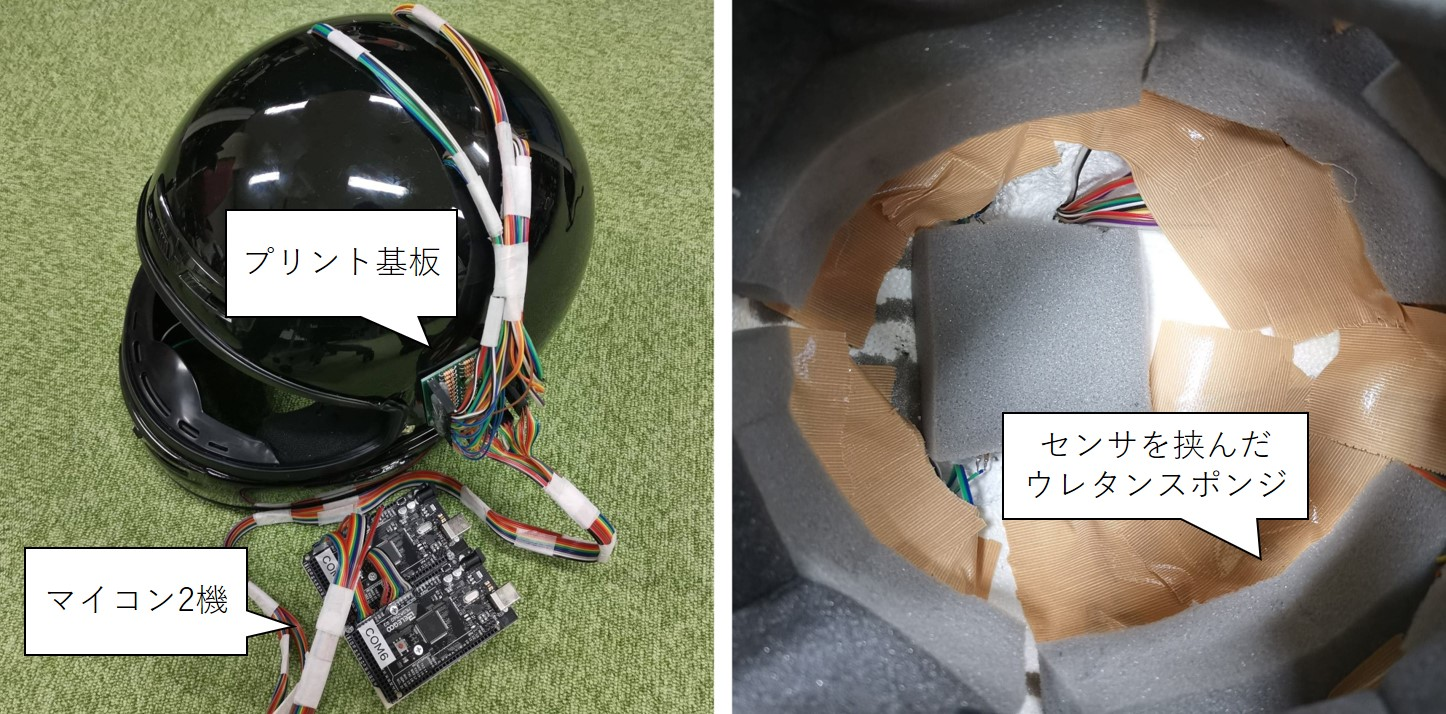
\includegraphics[width=1\linewidth]{met.eps}
  \end{center}
    \vspace{-8mm} 
  \caption{実装したプロトタイプデバイス}
  \label{device}
\end{figure}

\begin{figure}[!t]
  \begin{center}
    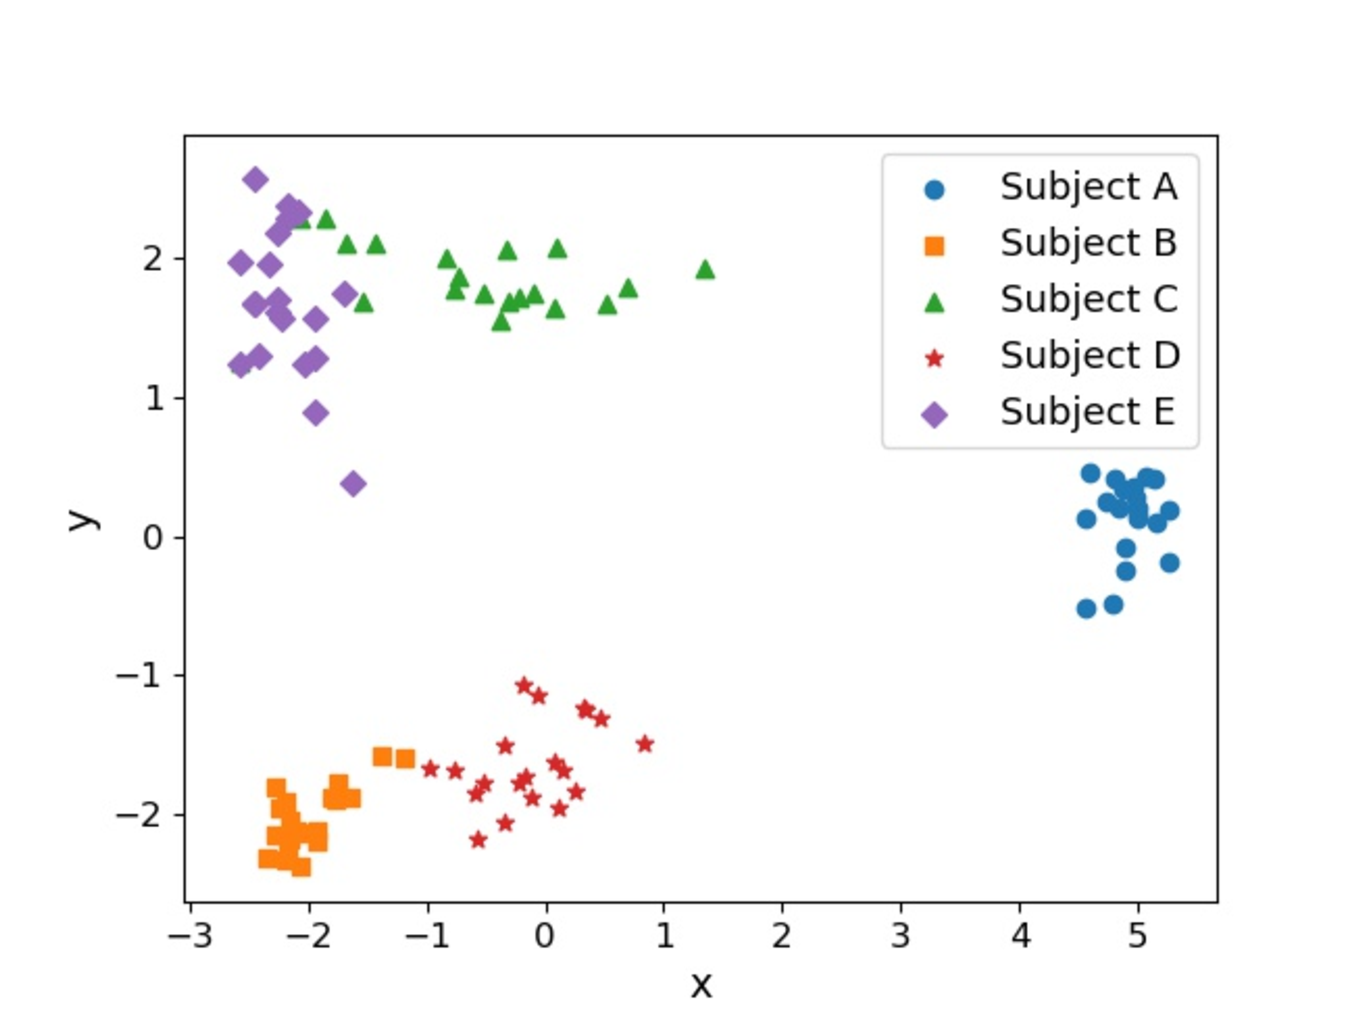
\includegraphics[width=1\linewidth]{PCA.eps}
  \end{center}
    \vspace{-8mm} 
  \caption{PCAによる分析結果}
  \label{pca}
\end{figure}

\begin{thebibliography}{2}
 \bibitem{bib1} 白川功浩,吉浦 裕,市野将嗣:虹彩および目の周辺の分割画像を用いた個人認証,情報処理学会論文誌,Vol. 59,No. 9,pp. 1726--1738 (2018).
%\bibitem{bib2} 新島有信,伊勢崎隆司,青木良輔,渡部智樹,山田智広:導電性高分子電極を用いた帽子型筋電センサの提案,電子情報通信学会論文誌D,Vol. J101-D,No. 10,pp. 1378-1387 (2018).
 \end{thebibliography}
\end{document}